\documentclass[12pt,letterpaper]{article}

% ===== Encoding and fonts =====
\usepackage[utf8]{inputenc}
\usepackage[T1]{fontenc}
\usepackage{mathptmx}
\usepackage{helvet}
\usepackage{courier}

% ===== Page geometry (zero margins) =====
\usepackage[top=0bp,bottom=0bp,left=0bp,right=0bp,headheight=0bp,headsep=0bp,footskip=0bp,paperwidth=612.00bp,paperheight=792.00bp]{geometry}

% ===== Packages =====
\usepackage[dvipsnames,svgnames,x11names]{xcolor}
\usepackage{graphicx}
\usepackage{tikz}
\usepackage{float}
\usepackage{amsmath}
\usepackage{amssymb}
\usepackage[normalem]{ulem}  % for \uline (underline)

% ===== No default spacing =====
\setlength{\parindent}{0pt}
\setlength{\parskip}{0pt}
\pagestyle{empty}

% ===== Custom colours =====
\definecolor{pdfcolor1}{RGB}{0,166,236}
\definecolor{pdfcolor2}{RGB}{255,108,197}
\definecolor{pdfcolor3}{RGB}{180,172,187}
\definecolor{pdfcolor4}{RGB}{201,201,201}
\definecolor{pdfcolor5}{RGB}{255,175,45}
\definecolor{pdfcolor6}{RGB}{0,210,106}
\definecolor{pdfcolor7}{RGB}{175,175,175}
\definecolor{pdfcolor8}{RGB}{232,232,232}

\begin{document}

\noindent
\begin{tikzpicture}[x=1bp,y=-1bp,inner sep=0pt,outer sep=0pt]
  \useasboundingbox (0,0) rectangle (612.00,792.00);
  \fill[fill=pdfcolor7] (72.00,107.75) rectangle (540.00,109.20);
  \fill[fill=pdfcolor7] (72.26,107.78) rectangle (539.97,108.02);
  \fill[fill=pdfcolor7] (72.02,108.02) rectangle (72.26,108.98);
  \fill[fill=pdfcolor8] (539.98,108.02) rectangle (540.22,108.98);
  \fill[fill=pdfcolor8] (72.26,108.98) rectangle (539.97,109.22);
  \fill[fill=pdfcolor7] (72.00,452.65) rectangle (540.00,454.10);
  \fill[fill=pdfcolor7] (72.26,452.78) rectangle (539.97,453.02);
  \fill[fill=pdfcolor7] (72.02,453.02) rectangle (72.26,453.98);
  \fill[fill=pdfcolor8] (539.98,453.02) rectangle (540.22,453.98);
  \fill[fill=pdfcolor8] (72.26,453.98) rectangle (539.97,454.22);
  \fill[fill=pdfcolor7] (72.00,684.00) rectangle (540.00,685.45);
  \fill[fill=pdfcolor7] (72.26,684.19) rectangle (539.97,684.43);
  \fill[fill=pdfcolor7] (72.02,684.43) rectangle (72.26,685.39);
  \fill[fill=pdfcolor8] (539.98,684.43) rectangle (540.22,685.39);
  \fill[fill=pdfcolor8] (72.26,685.39) rectangle (539.97,685.63);
  \node[anchor=north west,inner sep=0pt] at (72.00,267.20) {
\includegraphics[width=468.00bp,height=164.20bp]{images/image_p1_1.png}};
  \node[anchor=north west,inner sep=0pt] at (72.00,543.33) {
\includegraphics[width=468.00bp,height=127.50bp]{images/image_p1_2.png}};
  \node[anchor=north west,inner sep=0pt,outer sep=0pt] at (72.02,74.54) {\textsf{{\fontsize{12.0bp}{14.4bp}\selectfont Here's a }}\textsf{{\fontsize{12.0bp}{14.4bp}\selectfont \textbf{10-mark summarized answer}}}\textsf{{\fontsize{12.0bp}{14.4bp}\selectfont  on }}\textsf{{\fontsize{12.0bp}{14.4bp}\selectfont \textbf{Hebbian Learning}}}\textsf{{\fontsize{12.0bp}{14.4bp}\selectfont  based on the contents of your PDF: }}};
  \node[anchor=north west,inner sep=0pt,outer sep=0pt] at (72.02,125.62) {{\fontsize{12.0bp}{14.4bp}\selectfont \textcolor{pdfcolor1}{ }}\textsf{{\fontsize{12.0bp}{14.4bp}\selectfont \textbf{ Hebbian Learning – 10 Marks Summary }}}};
  \node[anchor=north west,inner sep=0pt,outer sep=0pt] at (72.02,152.26) {{\fontsize{12.0bp}{14.4bp}\selectfont \textcolor{pdfcolor2}{ }}\textsf{{\fontsize{12.0bp}{14.4bp}\selectfont \textbf{ Definition: }}}};
  \node[anchor=north west,inner sep=0pt,outer sep=0pt,text width=521.05bp] at (72.02,178.01) {\textsf{{\fontsize{12.0bp}{14.4bp}\selectfont Hebbian Learning is a }}\textsf{{\fontsize{12.0bp}{14.4bp}\selectfont \textbf{biologically inspired learning rule}}}\textsf{{\fontsize{12.0bp}{14.4bp}\selectfont  proposed by }}\textsf{{\fontsize{12.0bp}{14.4bp}\selectfont \textbf{Donald Hebb (1949)}}}\textsf{{\fontsize{12.0bp}{14.4bp}\selectfont . It }} \\
\textsf{{\fontsize{12.0bp}{14.4bp}\selectfont states: }}};
  \node[anchor=north west,inner sep=0pt,outer sep=0pt] at (72.02,219.79) {\textsf{{\fontsize{12.0bp}{14.4bp}\selectfont \textit{“When a neuron A repeatedly helps fire neuron B, the connection between them strengthens.”}}}\textsf{{\fontsize{12.0bp}{14.4bp}\selectfont  }}};
  \node[anchor=north west,inner sep=0pt,outer sep=0pt] at (72.02,244.75) {\textsf{{\fontsize{12.0bp}{14.4bp}\selectfont Mathematically, the change in weight is: }}};
  \node[anchor=north west,inner sep=0pt,outer sep=0pt] at (72.02,470.59) {{\fontsize{12.0bp}{14.4bp}\selectfont \textcolor{pdfcolor3}{ }}\textsf{{\fontsize{12.0bp}{14.4bp}\selectfont \textbf{ Working Principle: }}}};
  \node[anchor=north west,inner sep=0pt,outer sep=0pt,text width=374.23bp] at (90.02,494.26) {{\fontsize{10.1bp}{12.1bp}\selectfont •}\textsf{{\fontsize{10.1bp}{12.1bp}\selectfont  }}\textsf{{\fontsize{12.0bp}{14.4bp}\selectfont \textbf{Neurons}}}\textsf{{\fontsize{12.0bp}{14.4bp}\selectfont  strengthen their connection when activated together. }}};
  \node[anchor=north west,inner sep=0pt,outer sep=0pt,text width=106.95bp] at (90.02,519.22) {{\fontsize{10.1bp}{12.1bp}\selectfont •}\textsf{{\fontsize{10.1bp}{12.1bp}\selectfont  }}\textsf{{\fontsize{12.0bp}{14.4bp}\selectfont In vector form: }}};
  \node[anchor=north west,inner sep=0pt,outer sep=0pt] at (72.02,702.03) {{\fontsize{12.0bp}{14.4bp}\selectfont \textcolor{pdfcolor4}{ }}\textsf{{\fontsize{12.0bp}{14.4bp}\selectfont \textbf{ Key Properties: }}}};
\end{tikzpicture}
\newpage
\noindent
\begin{tikzpicture}[x=1bp,y=-1bp,inner sep=0pt,outer sep=0pt]
  \useasboundingbox (0,0) rectangle (612.00,792.00);
  \fill[fill=pdfcolor7] (72.00,157.70) rectangle (540.00,159.10);
  \fill[fill=pdfcolor7] (72.26,157.73) rectangle (539.97,157.97);
  \fill[fill=pdfcolor7] (72.02,157.97) rectangle (72.26,158.93);
  \fill[fill=pdfcolor8] (539.98,157.97) rectangle (540.22,158.93);
  \fill[fill=pdfcolor8] (72.26,158.93) rectangle (539.97,159.17);
  \fill[fill=pdfcolor7] (72.00,234.25) rectangle (540.00,235.70);
  \fill[fill=pdfcolor7] (72.26,234.31) rectangle (539.97,234.55);
  \fill[fill=pdfcolor7] (72.02,234.55) rectangle (72.26,235.51);
  \fill[fill=pdfcolor8] (539.98,234.55) rectangle (540.22,235.51);
  \fill[fill=pdfcolor8] (72.26,235.51) rectangle (539.97,235.75);
  \fill[fill=pdfcolor7] (72.00,432.25) rectangle (540.00,433.70);
  \fill[fill=pdfcolor7] (72.26,432.36) rectangle (539.97,432.60);
  \fill[fill=pdfcolor7] (72.02,432.60) rectangle (72.26,433.56);
  \fill[fill=pdfcolor8] (539.98,432.60) rectangle (540.22,433.56);
  \fill[fill=pdfcolor8] (72.26,433.56) rectangle (539.97,433.80);
  \fill[fill=pdfcolor7] (72.00,550.80) rectangle (540.00,552.25);
  \fill[fill=pdfcolor7] (72.26,550.97) rectangle (539.97,551.21);
  \fill[fill=pdfcolor7] (72.02,551.21) rectangle (72.26,552.17);
  \fill[fill=pdfcolor8] (539.98,551.21) rectangle (540.22,552.17);
  \fill[fill=pdfcolor8] (72.26,552.17) rectangle (539.97,552.41);
  \fill[fill=pdfcolor7] (72.00,702.25) rectangle (540.00,703.70);
  \fill[fill=pdfcolor7] (72.26,702.46) rectangle (539.97,702.70);
  \fill[fill=pdfcolor7] (72.02,702.70) rectangle (72.26,703.66);
  \fill[fill=pdfcolor8] (539.98,702.70) rectangle (540.22,703.66);
  \fill[fill=pdfcolor8] (72.26,703.66) rectangle (539.97,703.90);
  \node[anchor=north west,inner sep=0pt] at (108.00,325.14) {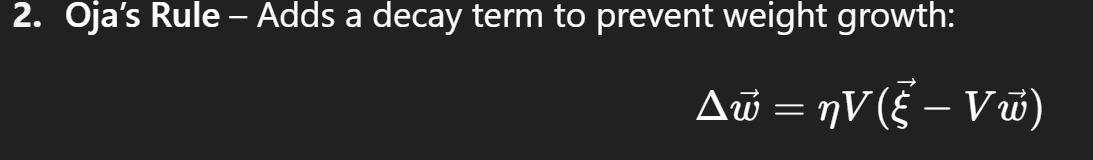
\includegraphics[width=468.00bp,height=68.50bp]{images/image_p2_3.png}};
  \node[anchor=north west,inner sep=0pt,outer sep=0pt] at (90.02,70.64) {\textsf{{\fontsize{12.0bp}{14.4bp}\selectfont 1.}}\textsf{{\fontsize{12.0bp}{14.4bp}\selectfont  }}\textsf{{\fontsize{12.0bp}{14.4bp}\selectfont \textbf{Unsupervised learning}}}\textsf{{\fontsize{12.0bp}{14.4bp}\selectfont  – no need for labeled output. }}};
  \node[anchor=north west,inner sep=0pt,outer sep=0pt] at (90.02,95.60) {\textsf{{\fontsize{12.0bp}{14.4bp}\selectfont 2.}}\textsf{{\fontsize{12.0bp}{14.4bp}\selectfont  }}\textsf{{\fontsize{12.0bp}{14.4bp}\selectfont \textbf{Locality}}}\textsf{{\fontsize{12.0bp}{14.4bp}\selectfont  – only uses data from connected neurons. }}};
  \node[anchor=north west,inner sep=0pt,outer sep=0pt] at (90.02,120.59) {\textsf{{\fontsize{12.0bp}{14.4bp}\selectfont 3.}}\textsf{{\fontsize{12.0bp}{14.4bp}\selectfont  }}\textsf{{\fontsize{12.0bp}{14.4bp}\selectfont \textbf{Biologically plausible}}}\textsf{{\fontsize{12.0bp}{14.4bp}\selectfont  – aligns with observed brain behavior. }}};
  \node[anchor=north west,inner sep=0pt,outer sep=0pt] at (72.02,175.54) {{\fontsize{12.0bp}{14.4bp}\selectfont \textcolor{pdfcolor5}{ }}\textsf{{\fontsize{12.0bp}{14.4bp}\selectfont \textbf{ Limitation: }}}};
  \node[anchor=north west,inner sep=0pt,outer sep=0pt,text width=421.43bp] at (90.02,199.23) {{\fontsize{10.1bp}{12.1bp}\selectfont •}\textsf{{\fontsize{10.1bp}{12.1bp}\selectfont  }}\textsf{{\fontsize{12.0bp}{14.4bp}\selectfont \textbf{Weight explosion}}}\textsf{{\fontsize{12.0bp}{14.4bp}\selectfont : Weights keep growing indefinitely unless controlled. }}};
  \node[anchor=north west,inner sep=0pt,outer sep=0pt] at (72.02,248.48) {{\fontsize{12.0bp}{14.4bp}\selectfont 🛠}\textsf{{\fontsize{12.0bp}{14.4bp}\selectfont \textbf{ Stabilization Techniques: }}}};
  \node[anchor=north west,inner sep=0pt,outer sep=0pt] at (90.02,273.97) {\textsf{{\fontsize{12.0bp}{14.4bp}\selectfont 1.}}\textsf{{\fontsize{12.0bp}{14.4bp}\selectfont  }}\textsf{{\fontsize{12.0bp}{14.4bp}\selectfont \textbf{Weight Normalization}}}\textsf{{\fontsize{12.0bp}{14.4bp}\selectfont  – Normalize the weight vector after each update. }}};
  \node[anchor=north west,inner sep=0pt,outer sep=0pt] at (90.02,298.96) {\textsf{{\fontsize{12.0bp}{14.4bp}\selectfont 2.}}\textsf{{\fontsize{12.0bp}{14.4bp}\selectfont  }}\textsf{{\fontsize{12.0bp}{14.4bp}\selectfont \textbf{Oja’s Rule}}}\textsf{{\fontsize{12.0bp}{14.4bp}\selectfont  – Adds a decay term to prevent weight growth: }}};
  \node[anchor=north west,inner sep=0pt,outer sep=0pt] at (90.02,381.54) {\textsf{{\fontsize{12.0bp}{14.4bp}\selectfont 3.}}\textsf{{\fontsize{12.0bp}{14.4bp}\selectfont  }}};
  \node[anchor=north west,inner sep=0pt,outer sep=0pt] at (108.05,399.12) {\textsf{{\fontsize{12.0bp}{14.4bp}\selectfont \textbf{Sejnowski’s Covariance Rule}}}\textsf{{\fontsize{12.0bp}{14.4bp}\selectfont  – Adjusts learning by subtracting the means. }}};
  \node[anchor=north west,inner sep=0pt,outer sep=0pt] at (72.02,450.19) {{\fontsize{12.0bp}{14.4bp}\selectfont \textcolor{pdfcolor1}{ }}\textsf{{\fontsize{12.0bp}{14.4bp}\selectfont \textbf{ Relation to PCA: }}}};
  \node[anchor=north west,inner sep=0pt,outer sep=0pt,text width=509.45bp] at (90.02,473.86) {{\fontsize{10.1bp}{12.1bp}\selectfont •}\textsf{{\fontsize{10.1bp}{12.1bp}\selectfont  }}\textsf{{\fontsize{12.0bp}{14.4bp}\selectfont Hebbian learning aligns the weight vector to the }}\textsf{{\fontsize{12.0bp}{14.4bp}\selectfont \textbf{direction of maximum variance}}}\textsf{{\fontsize{12.0bp}{14.4bp}\selectfont  in the }} \\
\textsf{{\fontsize{12.0bp}{14.4bp}\selectfont data. }}};
  \node[anchor=north west,inner sep=0pt,outer sep=0pt,text width=452.36bp] at (90.02,515.86) {{\fontsize{10.1bp}{12.1bp}\selectfont •}\textsf{{\fontsize{10.1bp}{12.1bp}\selectfont  }}\textsf{{\fontsize{12.0bp}{14.4bp}\selectfont This is the }}\textsf{{\fontsize{12.0bp}{14.4bp}\selectfont \textbf{first principal component}}}\textsf{{\fontsize{12.0bp}{14.4bp}\selectfont  in }}\textsf{{\fontsize{12.0bp}{14.4bp}\selectfont \textbf{Principal Component Analysis (PCA)}}}\textsf{{\fontsize{12.0bp}{14.4bp}\selectfont . }}};
  \node[anchor=north west,inner sep=0pt,outer sep=0pt] at (72.02,568.78) {{\fontsize{12.0bp}{14.4bp}\selectfont \textcolor{pdfcolor6}{ }}\textsf{{\fontsize{12.0bp}{14.4bp}\selectfont \textbf{ Applications: }}}};
  \node[anchor=north west,inner sep=0pt,outer sep=0pt,text width=118.82bp] at (90.02,592.45) {{\fontsize{10.1bp}{12.1bp}\selectfont •}\textsf{{\fontsize{10.1bp}{12.1bp}\selectfont  }}\textsf{{\fontsize{12.0bp}{14.4bp}\selectfont \textbf{Neural modeling}}}\textsf{{\fontsize{12.0bp}{14.4bp}\selectfont  }}};
  \node[anchor=north west,inner sep=0pt,outer sep=0pt,text width=128.48bp] at (90.02,617.43) {{\fontsize{10.1bp}{12.1bp}\selectfont •}\textsf{{\fontsize{10.1bp}{12.1bp}\selectfont  }}\textsf{{\fontsize{12.0bp}{14.4bp}\selectfont \textbf{Feature extraction}}}\textsf{{\fontsize{12.0bp}{14.4bp}\selectfont  }}};
  \node[anchor=north west,inner sep=0pt,outer sep=0pt,text width=192.27bp] at (90.02,642.39) {{\fontsize{10.1bp}{12.1bp}\selectfont •}\textsf{{\fontsize{10.1bp}{12.1bp}\selectfont  }}\textsf{{\fontsize{12.0bp}{14.4bp}\selectfont \textbf{Principal component learning}}}\textsf{{\fontsize{12.0bp}{14.4bp}\selectfont  }}};
  \node[anchor=north west,inner sep=0pt,outer sep=0pt,text width=298.57bp] at (90.02,667.35) {{\fontsize{10.1bp}{12.1bp}\selectfont •}\textsf{{\fontsize{10.1bp}{12.1bp}\selectfont  }}\textsf{{\fontsize{12.0bp}{14.4bp}\selectfont \textbf{Visual system simulations (e.g., Linsker's model)}}}\textsf{{\fontsize{12.0bp}{14.4bp}\selectfont  }}};
\end{tikzpicture}
\newpage
\noindent
\begin{tikzpicture}[x=1bp,y=-1bp,inner sep=0pt,outer sep=0pt]
  \useasboundingbox (0,0) rectangle (612.00,792.00);
  \node[anchor=north west,inner sep=0pt] at (72.00,96.97) {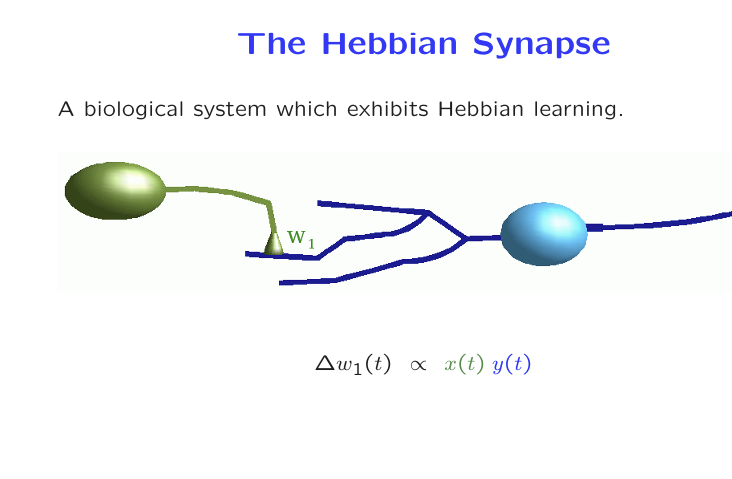
\includegraphics[width=468.00bp,height=306.25bp]{images/image_p3_4.png}};
  \node[anchor=north west,inner sep=0pt] at (72.00,405.54) {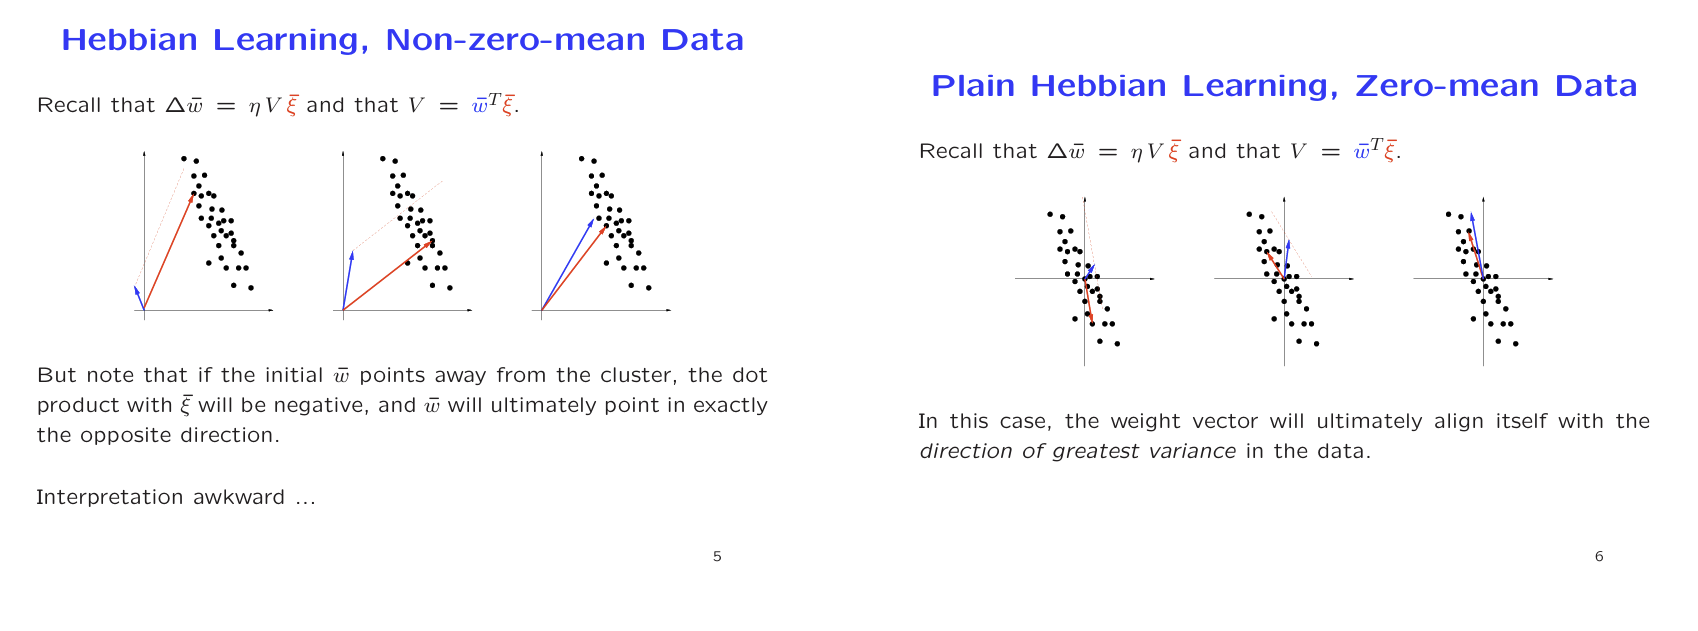
\includegraphics[width=468.00bp,height=173.90bp]{images/image_p3_5.png}};
  \node[anchor=north west,inner sep=0pt,outer sep=0pt] at (72.02,74.54) {\textsf{{\fontsize{12.0bp}{14.4bp}\selectfont Let me know if you'd like diagrams or a handwritten-style version for class notes! }}};
\end{tikzpicture}
\newpage
\noindent
\begin{tikzpicture}[x=1bp,y=-1bp,inner sep=0pt,outer sep=0pt]
  \useasboundingbox (0,0) rectangle (612.00,792.00);
  \node[anchor=north west,inner sep=0pt] at (72.00,72.00) {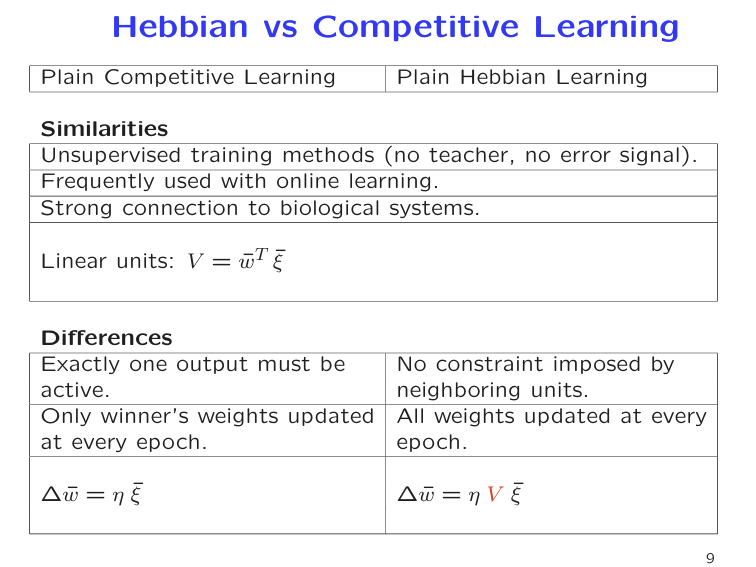
\includegraphics[width=468.00bp,height=351.00bp]{images/image_p4_6.png}};
\end{tikzpicture}

\end{document}
